\begin{code}[hide]
{-# OPTIONS --cubical --guardedness --no-import-sorts #-}

open import Cubical.Foundations.Prelude
open import Cubical.Data.Maybe using (Maybe)
\end{code}

Natural numbers are the initial object in the category of algebras over the
$\mathbb{1} + {-}$ endofunctor.

In the Agda proof assistant, it can be represented as an inductive datatype:

\begin{code}
data ℕ : Type where
  zero  : ℕ
  suc   : ℕ → ℕ
\end{code}

Dually, conatural numbers are the terminal object in the category of algebras
over the $\mathbb{1} + {-}$ endofunctor.

In Agda, it can be represented as a coinductive record type:

\begin{code}
record ℕ∞ : Type where
  coinductive
  field
    pred : Maybe ℕ∞
\end{code}

topological intuition

\begin{figure}[h]
  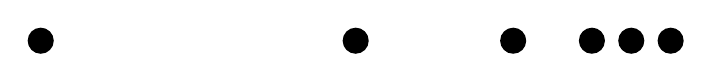
\begin{tikzpicture}[scale=8]
    \draw
      (0,0) node [shape=circle, fill] {}
      (0.5,0) node [shape=circle, fill] {}
      (0.75,0) node [shape=circle, fill] {}
      (0.875,0) node [shape=circle, fill] {}
      (0.9375,0) node [shape=circle, fill] {}
      (1,0) node [shape=circle, fill] {};
  \end{tikzpicture}
\end{figure}

failure of termination

\subsection{Related work}

sized types

decreasing boolean sequences

Naïm

TypeTopology
